\documentclass{article}

\usepackage[ngerman]{babel}
\usepackage{graphicx}
\usepackage{indentfirst}
\usepackage{hyperref}
\usepackage{geometry}
\usepackage{changepage}
\usepackage{booktabs}
\usepackage{float}
\usepackage{tabulary}
\usepackage{multirow}

\graphicspath{ {./images/} }
\setlength\parindent{0pt}

\makeatletter
\newcommand{\sectionauthor}[1]{
	{\parindent 0em \large \scshape Autor: #1 \par \nobreak \vspace*{1em}}
	\@afterheading
}
\newcommand{\specification}[3]{
	{\parindent 0.5em \hangindent 3em \hypertarget{spec:#1:#2}{\textbf{/#1#2/}} #3 \par \nobreak \vspace*{0.5em}}
}
\makeatother

\title{Bibliotheksanwendung - Feinspezifikation}
\date{\today\\v1.0}
\author{
	Ivan Charviakou\\
	León Liehr\\
	Mohamad Najjar\\
	Jonas Picker\\
	Sergei Pravdin
}

\begin{document}
\maketitle
\begin{figure}[h]
	\centering
	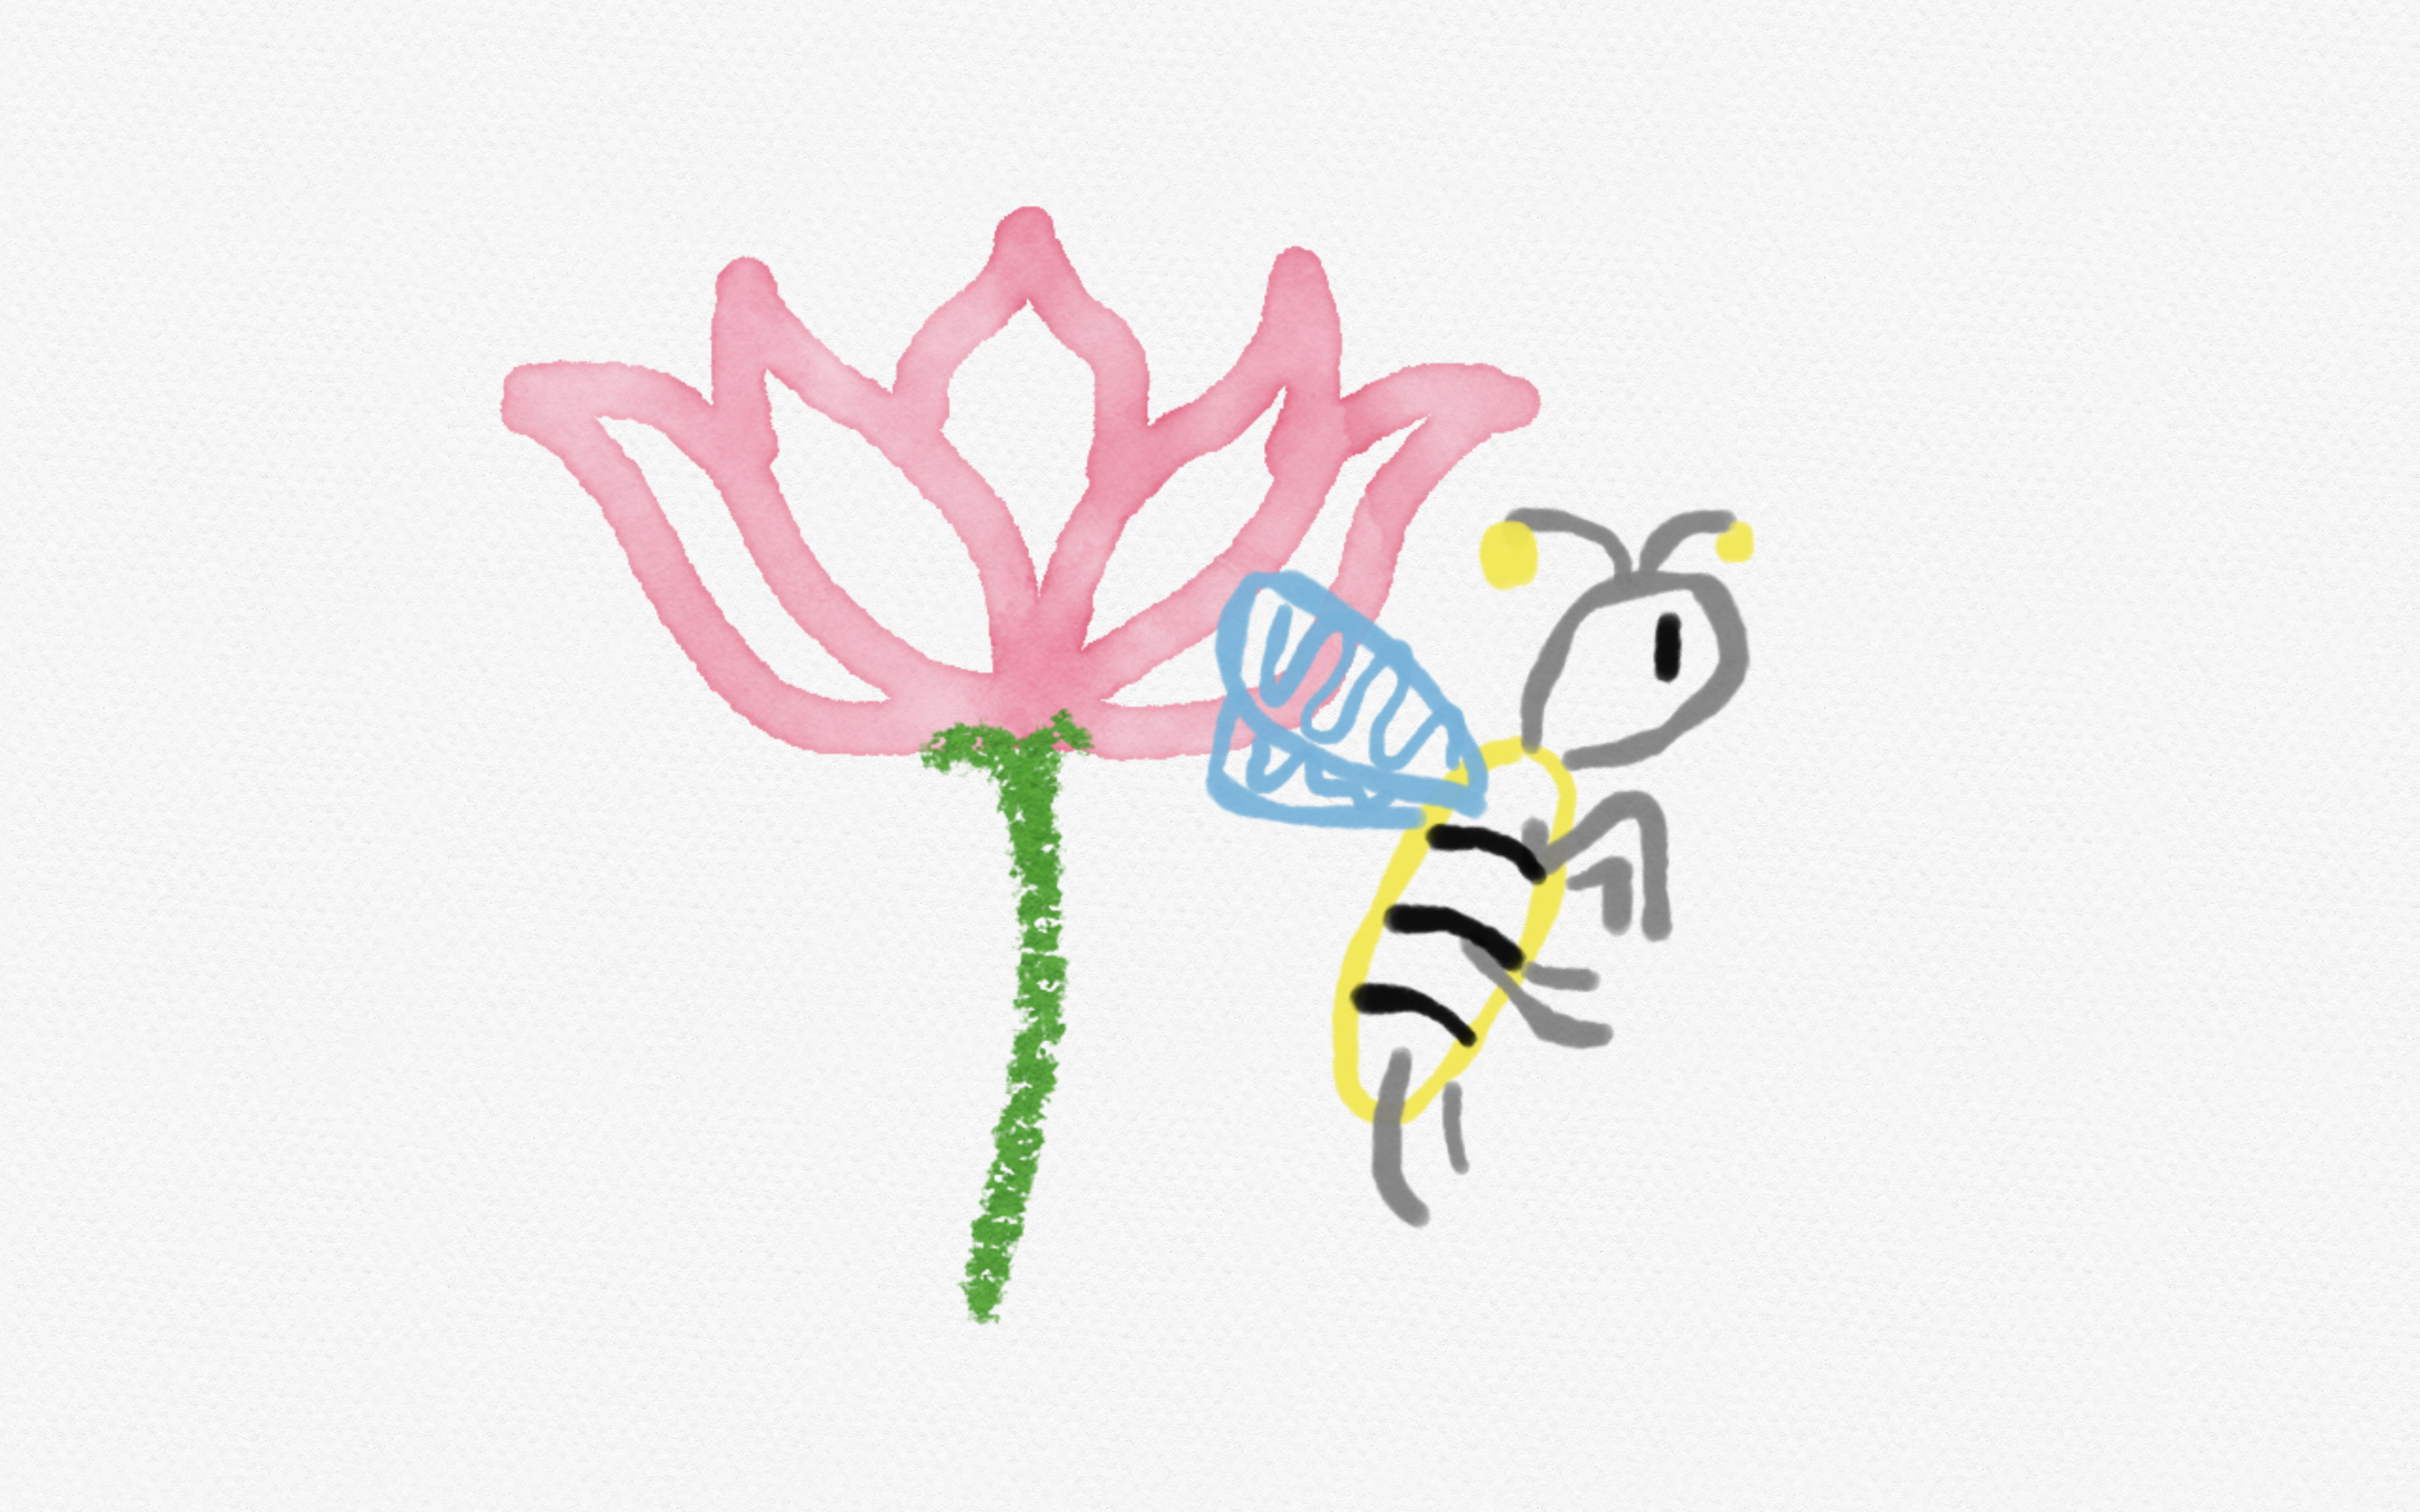
\includegraphics[width = 30em]{Logo}
\end{figure}
\newpage
\tableofcontents
\newpage

%----------------------------------------------------------------------Kapitel 1--------------------------------------------------------------------------------------------

\section{Einleitung}
Bei diesem Dokument handelt es sich um die Feinspezifikation unseres Bibliothekssystems. Es baut direkt auf dem vorangegangenen Entwurf auf und enthält einen noch genaueren Umriss der zu erstellenden Applikation.

%----------------------------------------------------------------------Kapitel 2--------------------------------------------------------------------------------------------

\section{Projektübersicht}
\sectionauthor{Ivan Charviakou}

\subsection{Paketübersicht und Ordnerstruktur}
Das angegebene Diagramm stellt die MVC-Architektur mit den Beziehungen zwischen den einzelnen Komponenten anhand der gegebenen Applikation dar. 
Dabei folgt die Komponentenaufteilung der Paketstruktur der Applikation und es werden die Paketnamen zusammen mit den wichtigsten darin enthaltenen Klassen / Komponenten / Funktionalitäten angegeben. 
Zudem entsprechen die Farben, die die Pakete im Diagramm besitzen, den Farben im nachfolgenden Klassendiagramm. \vspace{0.5em}

Die Ordnerstruktur des Projekts wird als Ordnerbaum dargestellt. 
Während die Paketstruktur im Ordner 'BiBi.src.main.java' abgebildet ist, enthält 'BiBi.src.main.webapp.view' die verwendeten Facelets mit entsprechender Rollenzuordnung. \vspace{0.5em}

\begin{figure}[h]

\end{figure}

\begin{figure}[h]
	\centering
	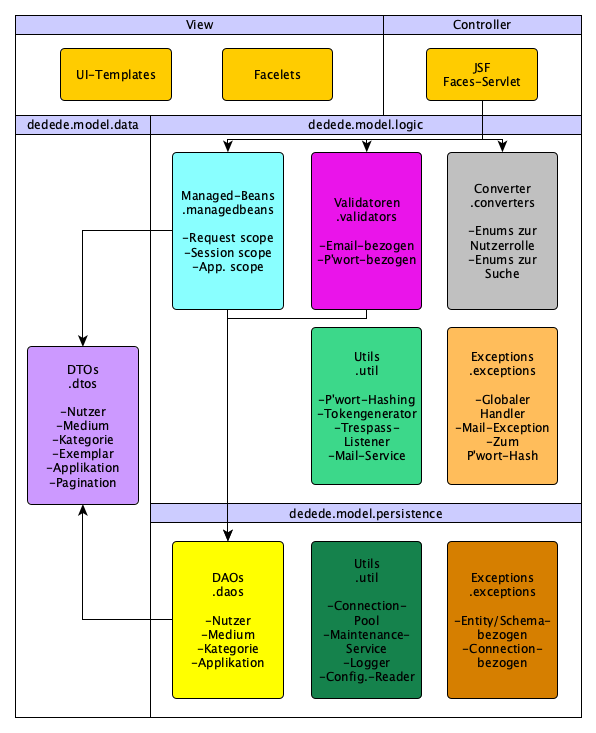
\includegraphics[width = 20em]{Modeldiagramm}
\end{figure}
\begin{figure}[h]
	\centering
	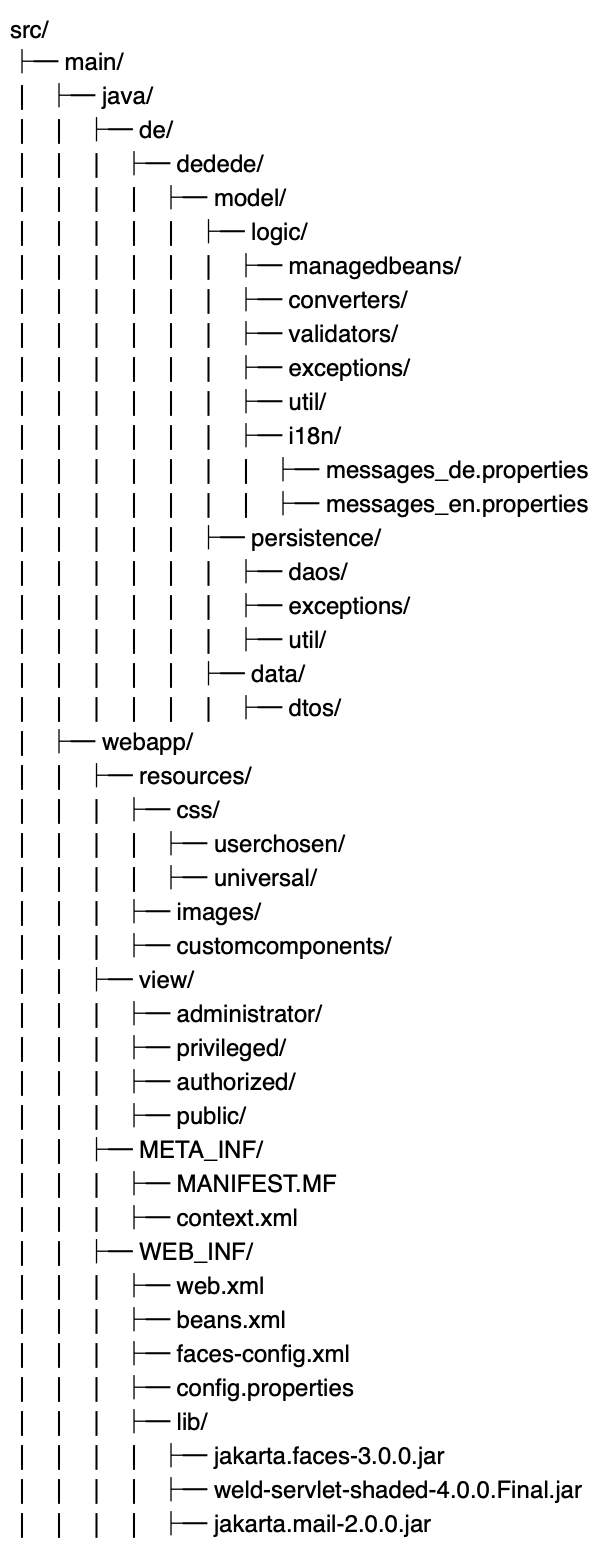
\includegraphics[width = 15em]{FileStructure}
\end{figure}

%----------------------------------------------------------------------Kapitel 3--------------------------------------------------------------------------------------------


%----------------------------------------------------------------------Kapitel 4--------------------------------------------------------------------------------------------
\newpage
\section{Bibliotheken}
\sectionauthor{Sergei Pravdin}

\newenvironment{controls}
{
    \begin{table}[H]
        \centering
        \begin{tabular}{ p{7em} p{19em} p{4em} p{12em} }
            \toprule
            \textbf{Bibliothek} & \textbf{Anwendungsbereich} & \textbf{Version} & \textbf{Lizenz}\\
            \midrule
        }
        {
            \bottomrule
        \end{tabular}
    \end{table}
}

Folgende Bibliotheken, bzw. Frameworks, werden für die Entwicklung unseres Bibliothekssystems verwendet.

\begin{controls}
    Jakarta Server Faces (JSF) & Grafische Benutzeroberflächen des Bibliotheksystems & 3.0.0 & GNU GPL / Java Community Process\\
    JDBC-Treiber für PostgreSQL & Integration des Bibliotheksystems mit der Datenbank & 42.2.20 & GNU GPL / Java Community Process\\
    JUnit & Testing & 5.7.1 & Common Public License\\
    Mockito & Testing & 3.9.0 & MIT-Lizenz\\
    PowerMock & Testing & 2.0.9 & Apache-Lizenz\\
    Selenium & Blackbox-Testing & 3.141.59 & Apache-Lizenz 2.0\\
    Apache Tomcat & Webserver & 10.0.2 & Apache-Lizenz 2.0\\
    Weld & Dependency Injection mittels Annotationen & 4.0.1 & Apache-Lizenz 2.0\\
    Jakarta Mail & Senden und Empfangen von E-Mails für die Verifizierung der Nutzers & 1.6.5 & CDDL 1.0, GPL 2.0, BSD\\
    Bootstrap & Anordnung der Frontend-CSS-Komponenten & 5.0.0 & MIT-Lizenz\\
\end{controls}

%----------------------------------------------------------------------Kapitel 5--------------------------------------------------------------------------------------------


%----------------------------------------------------------------------Kapitel 6--------------------------------------------------------------------------------------------


%----------------------------------------------------------------------Kapitel 7--------------------------------------------------------------------------------------------


%----------------------------------------------------------------------Kapitel 8--------------------------------------------------------------------------------------------
\newpage
\section{Datenfluss}
\sectionauthor{Sergei Pravdin}
Die Kommunikation zwischen den Klassen und die Interaktionen des Systems werden durch die Sequenzdiagramme abgebildet. Um einen Datenfluss beispielhaft zu zeigen, werden die folgenden beiden Szenarien vorgelegt: Zuerst bucht ein angemeldeter Nutzer ein Medium-Exemplar erfolgreich zur Ausleihe. Im zweiten Szenario bucht ein angemeldeter Nutzer ein Medium-Exemplar erfolglos zur Ausleihe, weil die Verbindung mit der Datenbank fehlgeschlagen ist. Das System ist so eingestellt, dass die angemeldeten Nutzer Zugriff auf die Medien haben. Der Nutzer möchte ein Exemplar des Mediums 'Programmieren lernen' buchen. Im System existiert das Medium mit dem Titel 'Programmieren lernen' und mit der Signatur (ID) '17RE'. Das Exemplar mit der Signatur (ID) '17RE (+1)' gehört zu dem genannten Medium und ist für eine Buchung verfügbar. Der Nutzer ruft die Mediumsseite 'medium.xhtml?id=17RE' auf.
\subsection{Interaktionen beim erfolgreichen Buchen eines Medium-Exemplars}
\subsubsection{Initialisierung der Mediumsseite}
Beim Laden der Mediumsseite wird die Methode 'init' als @PostConstruct zuerst aufgerufen. Die 'init'-Methode erzeugt ein Medium-DTO, das der Nutzer bekommt und setzt eine Medium-ID, die aus dem 'viewParam' kommt. Danach wird die 'viewAction()' durchgeführt, die die Mediumsseite durch die statische Methode aus dem Medium-DAO liefern muss. Das Medium-DAO bekommt auf der Datenschicht die Verbindung von der Singlton-ConnectionPool-Klasse durch die Methoden 'getInstance()' und 'getConnection()'. Im Körper der Methode 'loadMedium' wird eine SELECT-Anfrage durchgeführt, nachdem gibt das Medium-DAO die Verbindung durch die Methode 'releaseConnection' frei. Das Medium-DAO erfüllt mit erhaltenden von der Datenbank Attributen das Medium-DTO und gibt es dem Medium-BB zurück. Die Mediumsseite ist nun durch die Methode 'getAttributes' des Medium-DTOs komplett geladen.
\subsubsection{Buchen eines Exemplares}
Durch die Methode 'getCopies' des Medium-DTOs ist ein gewünschtes Exemplar dem Nutzer sichtbar. Der Nutzer klickt auf den Buchen-Button des Exemplars. Somit wird die Methode 'setCopyID' des Medium-DTOs aufgerufen, um die entsprechende ID festzulegen. Beim Klicken ruft der Nutzer die Methode 'fetchCopy' des Medium-BBs. Im Körper dieser Methode wird die Methode checkStatus() aus dem UserSession-BB aufgerufen, um zu prüfen, ob der Nutzer Zugriff auf die Funktion Buchen hat. Das UserSession-Bean meldet dem Medium-BB ein positives Ergebnis zurück. Das Medium-BB ruft die statische Methode MediumDAO.fetchCopy(mediumDTO) auf. Das Medium-DAO bekommt auf der Datenschicht die Verbindung von der Singlton-ConnectionPool-Klasse durch die Methoden 'getInstance()' und 'getConnection()'. Im Körper der Methode 'loadMedium' wird eine UPDATE-Anfrage durchgeführt, nachdem gibt das Medium-DAO die Verbindung durch die Methode 'releaseConnection' frei. Als Ergebnis der Methode 'fetchCopy' bekommt das Medium-BB das aktualisierte Medium-DTO. Der Nutzer bekommt eine Nachricht durch die statische Methode 'RessourceBandleHandler.getValue()' und die Buchung ist erfolgreich abgeschlossen.
\newgeometry{left=0cm,right=0cm,top=0cm,bottom=2cm}
\newpage
\begin{figure}[h]
    \centering
    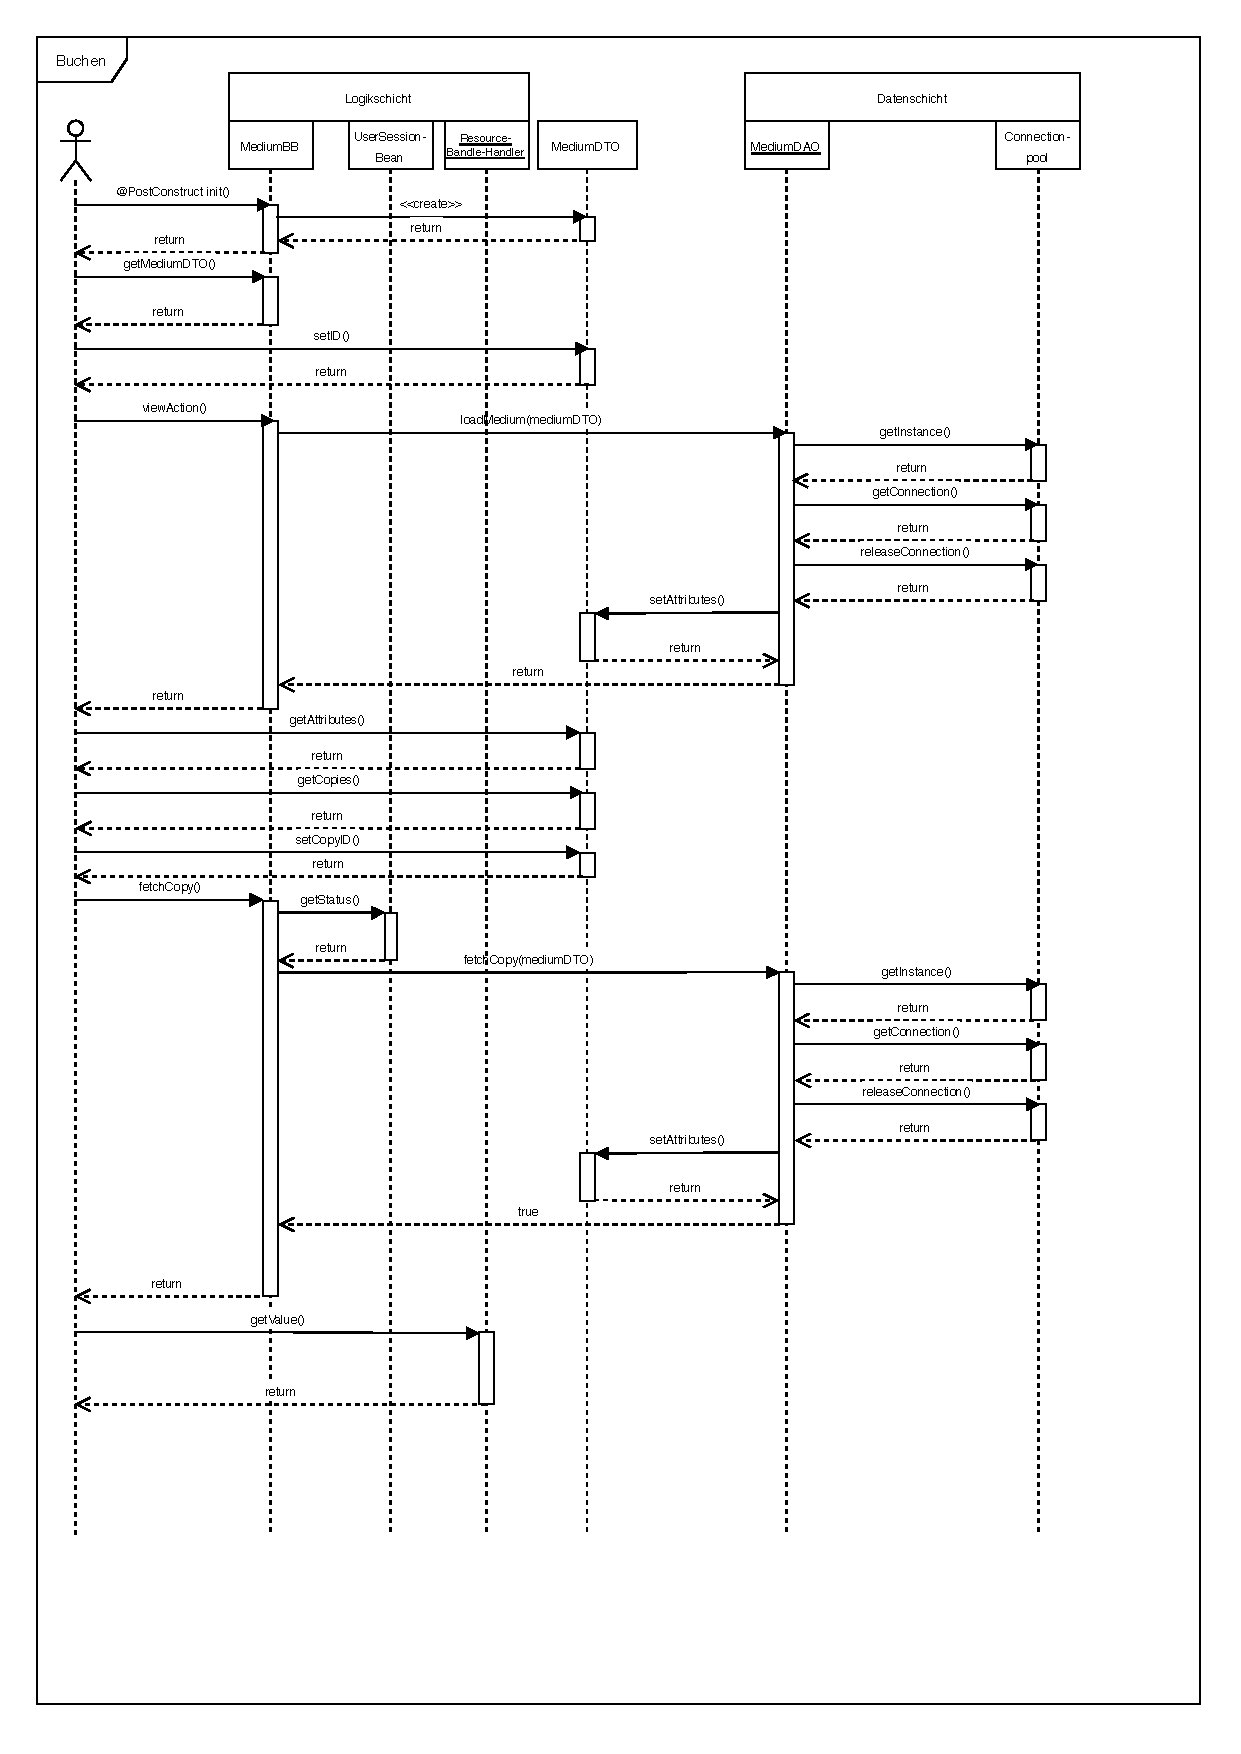
\includegraphics[width = 50em]{Sequenzdiagramm-success-v2}
    \caption{Interaktionen beim erfolgreichen Buchen eines Medium-Exemplares}
    \label{Sequenzdiagramm}
\end{figure}
\restoregeometry

\subsection{Interaktionen beim Buchen eines Medium-Exemplares mit fehlender Datenbankverbindung}
\subsubsection{Initialisierung der Mediumsseite}
Beim Laden der Mediumsseite wird die Methode 'init' als @PostConstruct zuerst aufgerufen. Die 'init'-Methode erzeugt ein Medium-DTO, das der Nutzer bekommt und setzt eine Medium-ID, die aus dem 'viewParam' kommt. Danach wird die 'viewAction()' durchgeführt, die die Mediumsseite durch die statische Methode aus dem Medium-DAO liefern muss. Das Medium-DAO bekommt auf der Datenschicht wegen technischen Problemen keine Verbindung von der Singlton-ConnectionPool-Klasse und die Methode 'getConnection' wirft einen SQLException. Das Medium-DAO wandelt den SQLException in den DataAccess-Exception um und wirft den dem Medium-BB. Mittels 'catch' ruft das Medium-BB die Methode 'handle' des ExceptionHandlers und das Exception-Handler schreibt den Fehler ins Loger durch 'addValue()' auf.
\subsubsection{Weiterleitung zur Fehlersseite}
Durch die Methode 'getValue()' des Exception-Handlers wird der Nutzer zur Fehlersseite weitergeleitet und bekommt von dem Resource-Bandle-Handler eine entsprechende Nachricht über den Fehler. Die Buchung ist nun erfolglos abgeschlossen.

\newpage

\newgeometry{left=0cm,right=0cm,top=0cm,bottom=2cm}

\begin{figure}[h]
	\hypertarget{Fehlersequenz}{}
    \centering
    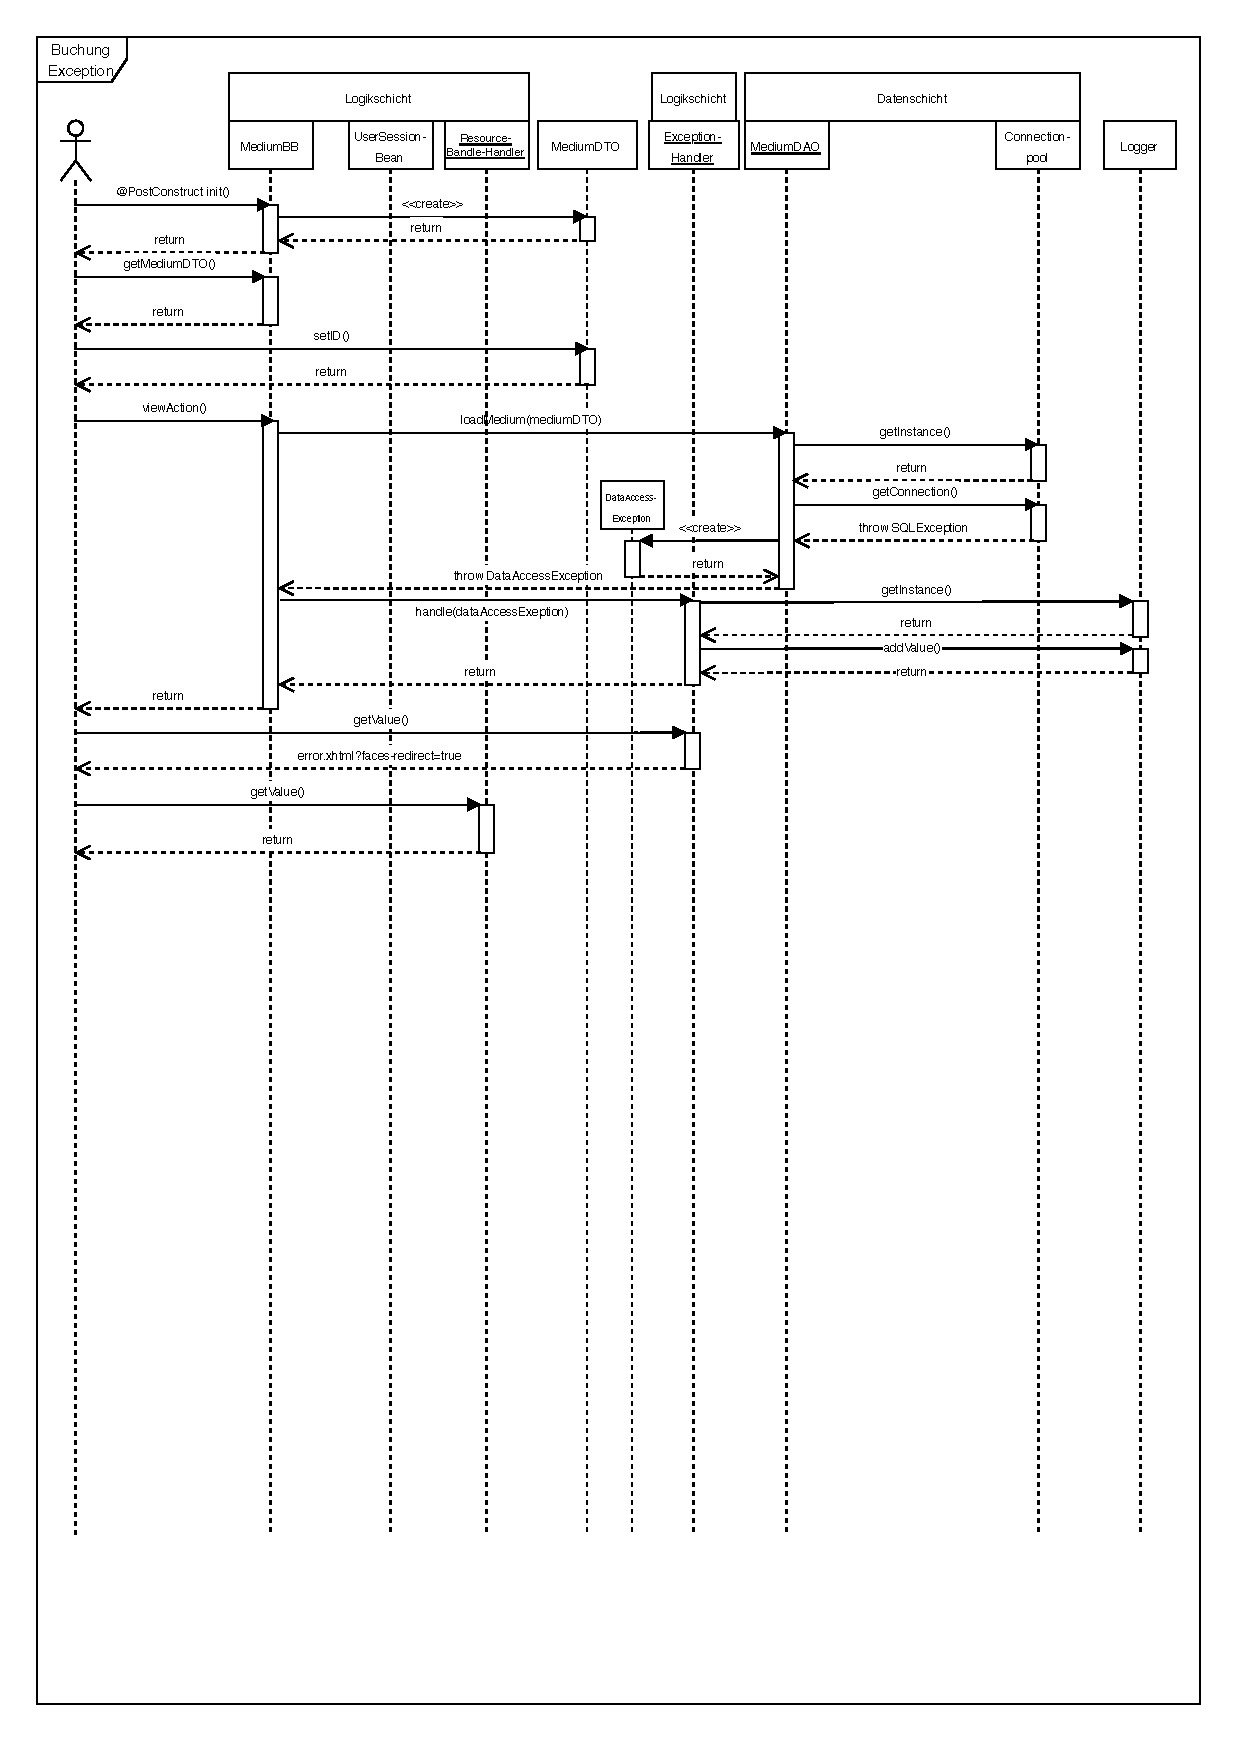
\includegraphics[width = 50em]{Sequenzdiagramm-exception-v3}
    \caption{Interaktionen beim Buchen eines Medium-Exemplares mit fehlender Datenbankverbindung}
    \label{Sequenzdiagramm}
\end{figure}

\restoregeometry
\newpage

%----------------------------------------------------------------------Kapitel 9--------------------------------------------------------------------------------------------


\end{document}